\documentclass{article}
\usepackage{graphicx}
\usepackage{amsmath}
\usepackage{pgfplots}
\usepackage{physics}
\usepackage{cancel}
\usepackage{bigints}
\usepackage{enumitem}
\usepackage{txfonts}
\usepackage[normalem]{ulem}

\newcommand{\g}{\text{g}}
\newcommand{\kilo}{\text{k}}
\newcommand{\m}{\text{m}}
\newcommand{\centi}{\text{c}}
\newcommand{\s}{\text{s}}
\newcommand{\N}{\text{N}}
\newcommand{\J}{\text{J}}
\newcommand{\C}{\text{C}}
\newcommand{\V}{\text{V}}
\newcommand{\A}{\text{A}}
\newcommand{\Ohm}{\text{\Omega}}

\pgfplotsset{compat=1.18}

\pgfplotsset{compat=1.18}

\usepackage[a4paper, top=1cm, bottom=2cm, left=2cm, right=2cm, includehead, includefoot]{geometry}



\begin{document}

\noindent
Physics 4B - Electromagnetism \hfill Prof. Alfred Cauthen
\noindent\rule{\textwidth}{0.4pt}

\begin{center}
    \textbf{\LARGE Homework 3} \\
    \vspace{12pt}
    \large Aaron W. Tarajos \\
    \textit{\today}
\end{center}

\noindent\rule{\textwidth}{0.4pt}

\section*{Chapter 22 Question 1}
Figure 22-22 shows three arrangements of electric field lines.
In each arrangement, a proton is released from rest at point A and is then accelerated through point B by the electric field. 
Points A and B have equal separations in the three arrangements. 
Rank the arrangements according to the linear momentum of the proton at point B, greatest first.

\begin{figure}[ht]
    \centering
    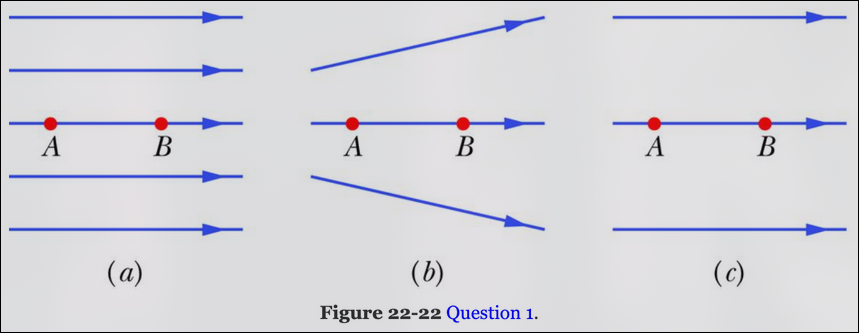
\includegraphics[scale=0.4]{image-1.png}
\end{figure}

\subsection*{Solution}
The ranking of the momentum at point $B$ is $a > b > c$ because the field lines are the most dense in $a$,  then are more dense at the beginning in $b$ but become equally less dense as in $c$ meaning there is greater initial force resulting in a higher momentum.

\section*{Chapter 22 Question 6}
In Fig. 22-27, two identical circular conducting rings are centeredon the same line with their planes perpendicular to the line. 
Each ringhas charge that is uniformly distributed along its circumference. 
The rings each produce electric fields at points along the line. 
For three situations, the charges on rings $A$ and $B$ are, respectively, (1) $q_0$ and $q_0$, (2) $-q_0$ and $-q_0$, and (3) $-q_0$ and $q_0$ . 
Rank the situations according to the magnitude of the net electric field at (a) point $P_1$ midway between the rings, (b) point $P_2$ at the center of ring B, and (c) point $P_3$ to the right of ring $B$, greatest first.

\begin{figure}[ht]
    \centering
    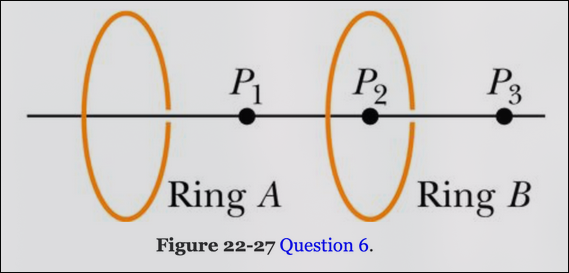
\includegraphics[scale=0.4]{image-2.png}
\end{figure}

\subsection*{Solution}
\textbf{Part a:} The ranking is $2 > 1 = 3$ because the electric field is the same from both rings but in opposite directions making the net field 0 except for when the charges are of the opposite sign in scenario 2
\[
	E_1 = \frac{Qd}{\left(R^2 + d^2\right)^{3/2}} - \frac{Qd}{\left(R^2 + d^2\right)^{3/2}} = 0
\]	
\textbf{Part b:} The magnitude of net field is the same in all scenarios because the field from ring $B$ will always be zero, and so we only have one field to consider and the sign does not affect magnitude;
\[
	E_2 = \frac{Q2d}{\left(R^2 + 4d^2\right)^{3/2}}
\]
\textbf{Part c:} The ranking is $1 = 2 > 3$ because the net field magnitude when the charges are the same are
\[
	E_3 = \frac{Q3d}{\left(R^2 + 9d^2\right)^{3/2}} +  \frac{Qd}{\left(R^2 + d^2\right)^{3/2}}
\]
and 
\[
	E_3^\prime = \frac{Qd}{\left(R^2 + d^2\right)^{3/2}} - \frac{Q3d}{\left(R^2 + 9d^2\right)^{3/2}}  
\]
when the charges are opposite.



\section*{Chapter 22 Question 9}
Figure 22-28 shows two disks and a flat ring, each with the same uniform charge $Q$. Rank the objects according to the magnitude of
the electric field they create at points $P$ (which are at the same vertical heights), greatest first.

\begin{figure}[ht]
    \centering
    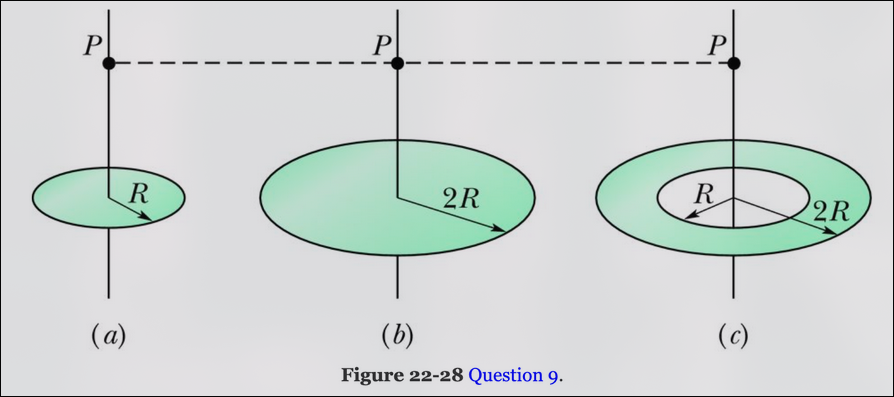
\includegraphics[scale=0.4]{image-3.png}
\end{figure}

\subsection*{Solution}
The ranking is $ a > c > b$. I was thinking about this one more intuitively and then showed it mathematically after I was already confident in my answer. We mostly care about the charge density of the different areas because the square root in the denominator of the second term makes changes in $R$ less significant than in the charge density.
\[
	E = \frac{\sigma}{2\epsilon_0} \left( 1 - \frac{z}{\sqrt{z^2 + R^2}}\right)
\]
where $\sigma$ is the charge density given by;
\[
	\sigma = \frac{Q}{\pi R^2}
\]
so as the area increases the charge density decreases. That of course means that $b$ will be the lowest, then something not completely obvious is that scenario $a$ has less area than $c$. Points within a circle are not uniformly distributed, meaning there are less points near the center than near the circumfrance and because there is less area we have a higher charge density. Now we can write out the terms for the net field of each to show this rigorously;
\[
	E_a = \frac{Q}{2\pi R^2\epsilon_0} \left( 1 - \frac{z}{\sqrt{z^2 + R^2}}\right)
\]
\[
	E_b = \frac{Q}{6\pi R^2\epsilon_0} \left( 1 - \frac{z}{\sqrt{z^2 + 4R^2}}\right)
\]
then $c$ is a little more challenging because we have to integrate;
\begin{align*}
	E_c &= \int_R^{2R} dE_c \\
		&= \frac{Q z}{4\epsilon_0} \int_R^{2R}\frac{2r}{\left(z^2 + r^2\right)^{3/2}} \ dr \\
		&= \frac{Qz}{4\epsilon_0} \left[\frac{-2}{\sqrt{z^2+r^2}}\right]_R^{2R} \\
		&= \frac{Qz}{4\epsilon_0 \left(4\pi R^2 -\pi R^2\right)} \left[\frac{-2}{\sqrt{z^2+4R^2}} + \frac{2}{\sqrt{z^2+R^2}}\right] 
\end{align*}

\section*{Chapter 22 Question 13}
Figure 22-32 shows three rods, each with the same charge $Q$ spread uniformly along its length. Rods $a$ (of length $L$) and $b$ (of
length $L/2$) are straight, and points $P$ are aligned with their midpoints. Rod $c$ (of length $L/2$) forms a complete circle about point $P$.
Rank the rods according to the magnitude of the electric field they create at points $P$, greatest first.

\begin{figure}[ht]
    \centering
    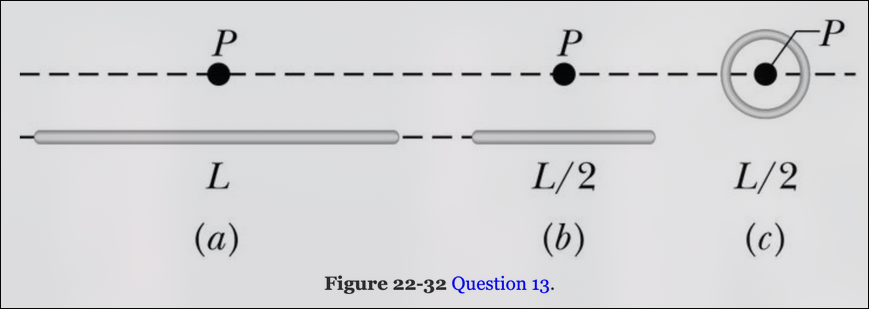
\includegraphics[scale=0.4]{image-4.png}
\end{figure}

\subsection*{Solution}
The ranking is $b > a > c$. Similar to the logic in the previous problem, $c$ has zero net field because the field from the ring cancels all around. Then for the $a$ and $b$ we only need to consider the vertical component of the field because the point is in the center of the rods so the horizontal components net to zero. We expect $b$ to be greater than $a$ because the the charge density is higher;

\[
	E_a = \frac{kQ}{L} \frac{L}{z\left(L^2 + z^2\right)^{1/2}}
\]
\[
	E_b = \frac{2kQ}{L} \frac{L}{2z\left(L^2/2 + z^2\right)^{1/2}}
\]
\section*{Chapter 22 Problem 24}
A thin nonconducting rod with a uniform distribution of positive charge $Q$ is bent into a complete circle of radius $R$. The central perpendicular axis through the ring is a $z$ axis, with the origin at the center of the ring. What is the magnitude of the electric field due to the rod at (a) $z = 0$ and (b) $z = \infty$? (c) In terms of $R$, at what positive value of $R$ is that magnitude maximum? (d) If $R = 2.00$ cm and $Q = 4.00$ $\mu$C, what is the maximum magnitude?

\begin{figure}[ht]
    \centering
    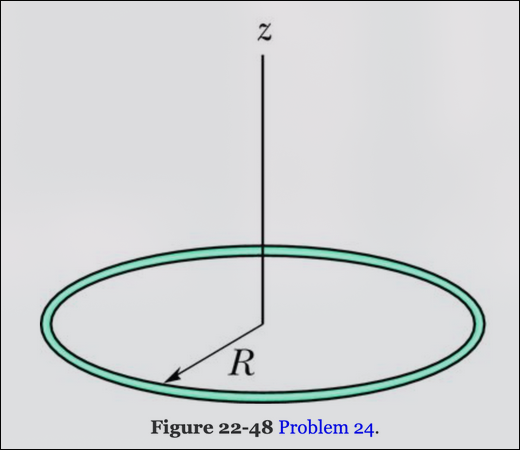
\includegraphics[scale=0.4]{image-5.png}
\end{figure}

\subsection*{Solution}
Consider the field at an arbitrary point $z$ perpendicular to a ring with a uniform charge distribution;
\[
	E = \frac{kQz}{\left(z^2+R^2\right)^{3/2}}
\]
\textbf{Part a:} It is clear that at $z=0$ the field is zero because of the term in the numerator.\\
\textbf{Part b:} The largest term involving $z$ is $z^2$ in the denominator which means that the deonminator will go to $\infty$ at a faster rate than the numerator where we only have $z$ and that means that in the limit the net field will also go to zero.\\
\textbf{Part c:} We take the derivative of the field equation;
\[
	\frac{d}{dz} \left[ \frac{kQz}{\left(z^2+R^2\right)^{3/2}} \right] = -\frac{Qk \left(2z^{2} - R^{2}\right)}{\left(z^{2} + R^{2}\right)^{\frac{5}{2}}}\]
then we set it equal to zero and solve for $z$;
\begin{align*}
	-\frac{Qk \left(2z^{2} - R^{2}\right)}{\left(z^{2} + R^{2}\right)^{\frac{5}{2}}} &= 0 \\
	Qk \left(2z^{2} - R^{2}\right) &=0 \\
	2z^2 - R^2 &= 0 \\
	2z^2 = R^2 \\
	z = \frac{R}{\sqrt{2}}
\end{align*}
\textbf{Part d:} At $R=2$ the maximum magnitude occurs at $z = \frac{2}{\sqrt{2}}$ at which we obtain a field magnitude of;
\[
	\frac{8.99 \times 10^9 \cdot 4 \times 10^{-6} \cdot \frac{2 \times 10^{-2}}{\sqrt{2}}}{\left(6 \times 10^{-4}\right)^{3/2}} = \boxed{3.460 \times 10^7 \ \N/\C}
\]

\section*{Chapter 22 Problem 26}
In Fig. 22-50, a thin glass rod forms a semicircle of radius $r = 5.00$ cm.
Charge is uniformly distributed along the rod, with $+q = 4.50$ pC in the upper half and $-q = -4.50$ pC in the lower half. 
What are the (a) magnitude and (b) direction (relative to the positive direction of the x axis) of the electric field E at P, the center of the semicircle?

\begin{figure}[ht]
    \centering
    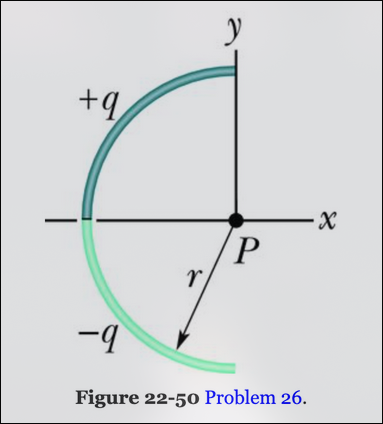
\includegraphics[scale=0.4]{image-6.png}
\end{figure}

\subsection*{Solution}
We can start by setting up this integral the same as for a standard ring.
\[
	E = \int dE
\]
but we only care about the vertical component because we can see that the horizontal components will be zero as they act in opposite directions.
\[
	E_y = \int dE \sin \theta
\]
and then we have
\begin{align*}
	E_y &= \int_0^{\pi/2} dE \sin \theta\\
	  &= \int_0^{\pi/2} k \frac{\lambda}{R} \sin \theta \ d\theta \\
	  &= \frac{k\lambda}{R} \left[-1 - 0\right] \\
	  &= -\frac{k\lambda}{R}
\end{align*}
that is just for the top half of the semi-circle, the total force then is just twice that since they act in the same direction;
\[
	-\frac{2\cdot 8.99\times10^9 \cdot 4.50 \times 10^{-12}}{\left(5 \times 10^{-2}\right)^2} = \boxed{-32.364\ \vu j \ \N/\C}
\]
\end{document}
